\section{Dead-Entry Miss Characterization}
\label{sec:characterization}

\subsection{Dead-Entry Ratio}
\label{sec:char_de_ratio}

Dead-entry misses are not a rare edge case but the dominant miss type across the
suite: 16 of 24 workloads exhibit dead-entry ratios above 90\%, and all 9
TLB-sensitive workloads exceed 98\% (six above 99\%). This near-unity ratio arises
because a TLB-sensitive workload's working set is large enough to force eviction
between successive accesses to the same page, yet small enough that the same
pages recur within a kernel -- so virtually every steady-state L2 miss re-walks a
page the TLB has already translated and discarded. High DE ratio alone does not
imply TLB sensitivity, however: \texttt{lud} and \texttt{gramschmidt} exceed 99\%
DE ratio yet sustain high throughput because their absolute miss rate is too low
for cumulative stall time to matter, motivating a joint condition of high DE
ratio \emph{and} high MPKI.

\begin{figure}[t]
  \centering
  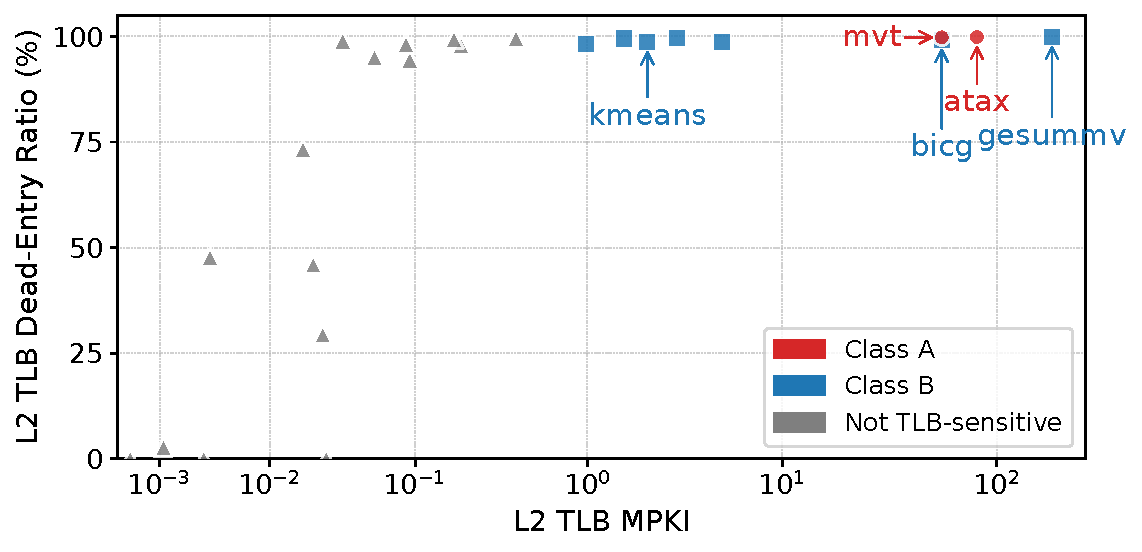
\includegraphics[width=\figwidth]{figs/fig04_de_ratio_vs_mpki.pdf}
  \caption{L2 TLB Dead-entry ratio vs.\ L2 TLB MPKI for all 24 workloads.}
  \label{fig:de_mpki}
\end{figure}

Figure~\ref{fig:de_mpki} plots all 24 workloads by DE ratio against MPKI. A
vertical gap separates the 9 TLB-sensitive workloads, at elevated MPKI, from the
other 15, and within that high-MPKI band every workload clusters near 100\% DE
ratio -- confirming near-unity DE ratio as a reliable marker of TLB-sensitive
steady state. Below the gap, DE ratio spans near-zero to above 99\% with no
relation to MPKI, confirming it carries no predictive power on its own.

\subsection{Access Structure: The Class Discriminator}
\label{sec:char_burstness}

\texttt{atax} and \texttt{bicg} illustrate why miss statistics alone are
insufficient: they share nearly identical DE ratios ($\sim$99.9\%/$\sim$99.2\%)
and comparable MPKI (81/56), and even their miss arrival rates track closely
through steady state, yet their response to the same eviction-history protection
differs by nearly two orders of magnitude. The discriminator is access
structure -- whether warps reference the same virtual page or distinct pages at
a given moment -- and Figure~\ref{fig:burstness} makes it visible directly:
\texttt{atax} shows brief, high-amplitude occupancy bursts, while \texttt{bicg}
is flat and sustained throughout.

\begin{figure}[ht]
  \centering
  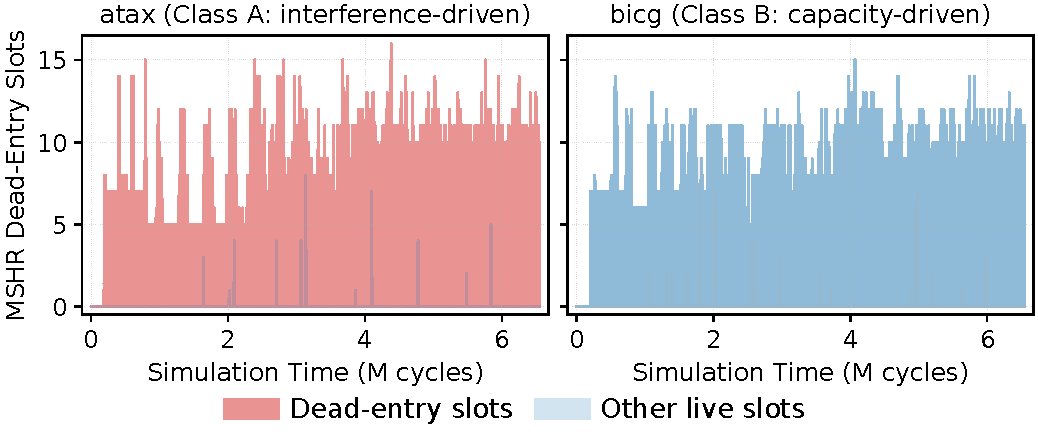
\includegraphics[width=\figwidth]{figs/fig06_mshr_burstness.pdf}
  \caption{MSHR dead-slot occupancy over time for \texttt{atax} and \texttt{bicg}.}
  \label{fig:burstness}
\end{figure}

In \texttt{atax}, each warp computes $y \mathrel{+}= A[i][j] \cdot x[j]$: all 32
threads access the same element of $x[]$, producing one shared VPN per warp
instruction. When that VPN is evicted and re-walked, every warp stalled on it
merges into a single MSHR entry, so one page walk releases many warps at once,
producing the sharp spikes in Figure~\ref{fig:burstness} (spike height tracks
merge depth); \texttt{mvt} shares this pattern for analogous algebraic reasons,
forming Class~A's second member. In \texttt{bicg}, each warp computes a column
dot product where thread $i$ accesses row $i$ of $A$, producing 32 distinct VPNs
per warp instruction with a merge depth near one -- its 2048-by-2048 working set
needs $\sim$4096 pages, four times L2 TLB capacity, so evictions are
capacity-driven and the occupancy trace stays flat, a structure shared by the
remaining six Class~B workloads (\texttt{nw}, \texttt{sssp}, \texttt{kmeans},
\texttt{gesummv}, \texttt{dmr}, \texttt{mst}). The two classes are thus
distinguished by occupancy shape alone -- bursty spikes mean shared pages and
disproportionate per-eviction recovery, flat sustained occupancy means
capacity-bound evictions no replacement policy can resolve -- observable from
existing MSHR counters with no offline profiling required.

\subsection{Validating Capacity-Driven Misses}
\label{sec:char_2mb}

If the seven Class~B workloads are genuinely capacity-driven, expanding TLB
reach should eliminate their dead-entry misses. Figure~\ref{fig:de_2mb} shows
IPC speedup under 2\,MB huge pages (L2 reach $4\,\text{MB}\rightarrow256\,\text{MB}$)
over the 4\,KB baseline for all nine TLB-sensitive workloads.

\begin{figure}[ht]
  \centering
  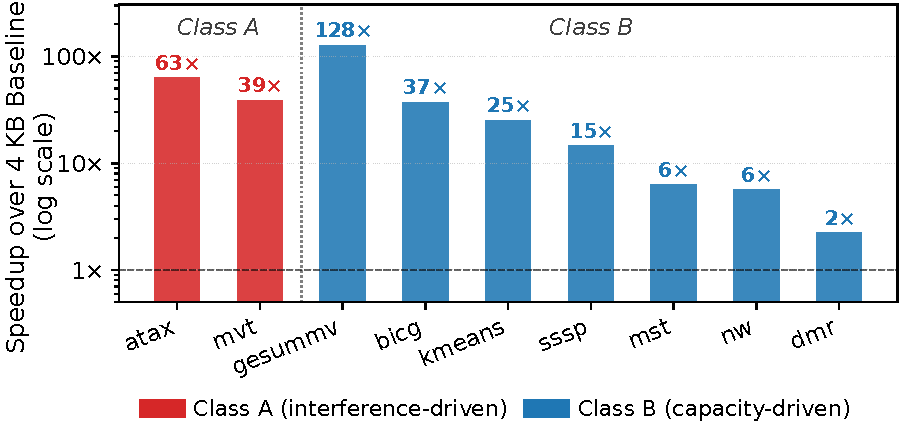
\includegraphics[width=\figwidth]{figs/fig07_2mb_ipc_speedup.pdf}
  \caption{IPC speedup under 2\,MB pages over 4\,KB baseline for all 9 TLB-sensitive workloads.}
  \label{fig:de_2mb}
\end{figure}

Results confirm the diagnosis for all 7 Class~B workloads, with speedups
tracking working-set size relative to the expanded reach: \texttt{gesummv}
$128\times$ (16\,MB set fits entirely), \texttt{bicg} $37\times$, \texttt{kmeans}
$25\times$, \texttt{sssp} $14.5\times$, \texttt{mst} $6.3\times$, \texttt{nw}
$5.7\times$, and \texttt{dmr} $2.2\times$ (a more irregular address stream, only
partially contained). Class~A also benefits substantially (\texttt{atax}
$63\times$, \texttt{mvt} $39\times$), but unlike Class~B, its performance is not
fundamentally capacity-constrained -- expanding reach does not eliminate the
interference among warps competing for the same entries.
